% =========================================================================== %
% Yes. This is a document.

\documentclass[
	english,
	aspectratio=169,
	table
]{beamer}

% =========================================================================== %
% Theme

\usepackage{scrlfile}
	\ReplacePackage{beamerthemeSHUR}{./sty/beamerthemeSHUR}
	\ReplacePackage{beamerinnerthemefancy}{./sty/beamerinnerthemefancy}
	\ReplacePackage{beamerouterthemedecolines}{./sty/beamerouterthemedecolines}
	\ReplacePackage{beamercolorthemechameleon}{./sty/beamercolorthemechameleon}

\usetheme[
	pageofpages=von,
	bullet=circle,
	titleline=true,
	alternativetitlepage=true,
	watermark="",
	watermarkheight=0px,
	watermarkheightmult=0
	]
{SHUR}

% =================================================================================================== %
% the usual stuff

\usepackage[utf8]{inputenc}
\usepackage[T1]{fontenc}
\usepackage{babel}
\usepackage{lmodern}
\usepackage{microtype}
\usepackage{csquotes}
\usepackage{xspace}
%\usepackage{ragged2e}

\usepackage{tabularx}
\usepackage{booktabs}
\usepackage{multirow}

\usepackage{color, colortbl}
\usepackage{xcolor}
	\definecolor{highlight}{RGB}{0,64,128}
	\setbeamercolor{alerted text}{fg=highlight,bg=}

\usepackage{tabto}
	
% math
\usepackage{amsmath}
\usepackage{amssymb}
\usepackage{dsfont}
\usepackage{mathtools}

\let\olddiv\div
\usepackage[arrowdel]{physics}

\usepackage{minted}
	\usemintedstyle{xcode}

\usepackage{tikz}
	\usetikzlibrary{positioning}
	\usetikzlibrary{matrix}
	\usetikzlibrary{shapes.geometric}
	\usetikzlibrary{backgrounds}
	\usetikzlibrary{calc}
	\usetikzlibrary{decorations.pathreplacing}
	\tikzstyle{every picture}+=[remember picture] 
\usepackage{adjustbox}

\usepackage{tcolorbox}
	\newtcolorbox{codebox}[1][Code]
		{colback=black!5!white,colframe=blue!40!black,title=#1,leftupper=7mm}
	\newtcolorbox{warnbox}[1][Beachte]
		{colback=black!5!white,colframe=red!40!black,title=#1}
	\newtcolorbox{hintbox}[1][Tipp]
		{colback=black!5!white,colframe=green!40!black,title=#1}
	\newenvironment{itembox}[1][]
		{\begin{tcolorbox}[title=#1]\begin{itemize}}{\end{itemize}\end{tcolorbox}}
	\newtcolorbox{doublebox}[1][.3]{
		righthand width=#1\linewidth,
		sidebyside,
		sidebyside gap=6mm,
		sidebyside align=center,
		lower separated=false}
	\tcbsetforeverylayer{colback=cyan!10!white,colframe=cyan!75!black}

\usepackage[super]{nth}

%==============================================================================%
% GLOBAL MACROS

%\addtokomafont{labelinglabel}{\sffamily}

\newcommand*{\tabcrlf}{\\ \hline}			% actually still allows for optional argument

% text elements
\newcommand*{\TODO}[1][!]{{\color{red} TODO #1}}

\newcommand*{\ie}{i.\,e.\xspace}
\newcommand*{\eg}{e.\,g.\xspace}

\newcommand*{\thus}{\ensuremath{\rightarrow}\xspace}
\newcommand*{\Thus}{\ensuremath{\Rightarrow}\xspace}

\newcommand*{\smallfrac}  [2]{\ensuremath{{}^        {#1} \!/_        {#2}}}
\newcommand*{\smallfracrm}[2]{\ensuremath{{}^{\mathrm{#1}}\!/_{\mathrm{#2}}}}

% generic maths
\newcommand*{\iunit}{\mathsf{i}}

\newcommand*{\mean}[1]{\overline{#1}}
\newcommand*{\conj}[1]{{#1}^{*}}
\newcommand*{\transp}{\ensuremath{^\top}}

\newcommand*{\ceil} [1]{\left\lceil {#1} \right\rceil }
\newcommand*{\floor}[1]{\left\lfloor{#1} \right\rfloor}

\DeclareMathOperator{\perm}{perm}
\DeclareMathOperator{\sign}{sign}
\DeclareMathOperator{\diag}{diag}

\newcommand*{\DD}[1]{\ensuremath{\text{D}\vec{#1}\;}}
\newcommand*{\set}[1]{\ensuremath{\{#1\}}}

% standard sets
\newcommand*{\setNaturals}{\mathds{N}}
\newcommand*{\setIntegers}{\mathds{Z}}
\newcommand*{\setReals}   {\mathds{R}}
\newcommand*{\setComplex} {\mathds{C}}

% physics
\newcommand*{\cre}[1][a]{\ensuremath{{\hat{#1}}^{\dagger}}}

\newcommand*{\vac}{\ensuremath{\ket{\text{vac}}}\xspace}
\newcommand*{\ketIn}{\ensuremath{\ket{\Psi}}\xspace}
\newcommand*{\ketOut}{\ensuremath{\ket{\Phi}}\xspace}
\newcommand*{\opU}{\ensuremath{\hat{U}}\xspace}
\newcommand*{\matU}{\ensuremath{\mathbb{U}}\xspace}
\newcommand*{\DFT}{\ensuremath{\mathbb{W}}\xspace}
\newcommand*{\sysArgs}{\vec{m}, \vec{n}; \matU}

% CS
\newcommand*{\bigo}[1]{\ensuremath{\mathcal{O}(#1)}\xspace}

\newcommand*{\inPy}[1]{\mintinline{python3}{#1}}
\newcommand*{\inCPP}[1]{\mintinline{c++}{#1}}

% =========================================================================== %

\author{\vspace{8pt}
Master Thesis Project Progress Report\newline 
Stefan Hartinger}
\title{Simulating Quantum Supremacy in a Classical Computer\vspace{8pt}}
\subtitle{Numerical Implementation of BosonSampling}
\institute{Universität Regensburg\newline Department Theoretical Physics}
\date{2021-06-02}

% =========================================================================== %

\begin{document}
% =========================================================================== %

\begin{frame}[t,plain]
\titlepage
\end{frame}

% =========================================================================== %

\begin{frame}{Computing the Permanent -- A Computationally Hard Problem}
%
\begin{align*}
	\perm(\mathbb{A})
&\coloneqq
	\sum_{\sigma \in S_N} \prod_{j=1}^{N} a_{i, \sigma(j)}
&&
	\text{where}
&
	\mqty{
		A = (a_{ij}) \in \setComplex^{N \times N} \\
		S_N : \text{symmetric group of size } N \\
	}
\end{align*}
%
\begin{itemize}
\item Use as bosonic equivalent to Slater Determinant
\item Direct evaluation takes $\bigo{N!N}$ FLOPs -- compuatationally extremely hard\\
	(sign problem)
\item[\Thus] Bosonic systems can be used to \enquote{measure} the permanent
\item[\Thus] Quantum Supremacy
\item Need for Certification
\end{itemize}
%
\end{frame}

% =========================================================================== %

\begin{frame}{The Hong-Ou-Mandel Effect: Observation}
%
\begin{columns}[t]
\column{.5\linewidth}
\begin{itemize}
\item Pair of \emph{identical} photons %from SPDC (\emph{spontaneous parametric down-conversion})
\item Beam Splitter: T/R-Ratio 50:50
\item Classical Particles: 1:2:1 in occupations (2,0), (1,1), (0,2)
\item Photons: 1:1 in occupations (2,0), (0,2)
\item[\Thus] Surpression of one outcome due to interference
\end{itemize}
%
\column{.5\linewidth}
\begin{figure}
	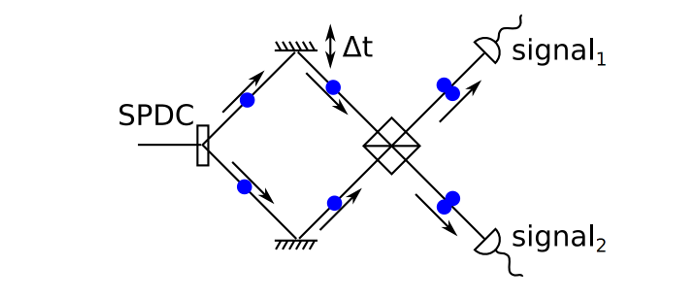
\includegraphics[height=2.5cm]{./gfx/HOM-simple}\hspace{200pt}	
	%
	\begin{flushleft}
		\footnotesize Hong-Ou-Mandel Effect, Experimental Setup, schematic.
	\end{flushleft}
	%
\end{figure}
\end{columns}

\vspace{30pt}
{\scriptsize 
	Image Source: \url{www.qutools.com/qued/qued-sample-experiments/sample-experiments-hong-ou-mandel/}
}
%
\end{frame}

% =========================================================================== %

\begin{frame}[t]{The Hong-Ou-Mandel Effect: QM Explanation}
%
\begin{itemize}
\item Coherent photons \Thus shared wave function
	\tabto{7cm} $ \ketIn  = \qty( \prod_j \cre[a]_j ) \vac $
\item Assume: system does not break coherence
	\tabto{7cm} $ \ketOut = \qty( \prod_j \cre[b]_j ) \vac $
\item	Time evolution operator
	\tabto{7cm} $ \ketOut = \opU \ketIn $
\item With effect
	\tabto{7cm} $ \cre_j \to \opU \cre_j \opU^{-1} = \iunit \sqrt{R} \cre[b]_j + \sqrt{T} \cre[b]_{3-j} $
\item Phase shift by $\iunit$ from reflection
\item Multiply out and apply bosonic commutator rule $\cre[b]_1 \cre[b]_2 = \cre[b]_2 \cre[b]_1$:
	\begin{align*}
		\textstyle
		\ketOut
	&=
		\opU \ketIn = \opU \cre_1 \cre_2 \vac \\
%	&=
%		\qty(
%			(\iunit \sqrt{R} \cre[b]_1 + \sqrt{T} \cre[b]_2)
%			(\iunit \sqrt{R} \cre[b]_2 + \sqrt{T} \cre[b]_1)
%		) \vac \\
%	&=
%		\qty(
%			+ \iunit \sqrt{RT} (\cre[b]_1)^2
%			+ \iunit \sqrt{RT} (\cre[b]_2)^2
%			+ T \cre[b]_2 \cre[b]_1
%			- R \cre[b]_1 \cre[b]_2
%		) \vac \\
	&=
		\qty(
			+ \iunit \sqrt{RT} (\cre[b]_1)^2
			+ \iunit \sqrt{RT} (\cre[b]_2)^2
			+ (T - R) \cre[b]_2 \cre[b]_1
		) \vac
	\end{align*}
\end{itemize}
%
\end{frame}

% =========================================================================== %

\begin{frame}[t]{The Hong-Ou-Mandel Effect: Generalization}
%
\begin{columns}
\column{.75\linewidth}
\begin{itemize}
\item Express as Linear Transformation
	\begin{align*}
		\begin{pmatrix}
			\cre_1 \\
			\cre_2
		\end{pmatrix}
	\xrightarrow{\opU}
		\begin{pmatrix}
			\sqrt{R} &  \sqrt{T} \\
			\sqrt{T} & -\sqrt{R}
		\end{pmatrix}
		\begin{pmatrix}
			\cre[b]_1 \\
			\cre[b]_2
		\end{pmatrix}
	\end{align*}
\item Introduce \emph{Phase Shifting Devices}
	\begin{align*}
		\begin{pmatrix}
			\cre_1 \\
			\cre_2
		\end{pmatrix}
	\xrightarrow{\opU}
		\begin{pmatrix}
			\sqrt{R} & +\sqrt{T} \exp(\iunit \phi)  \\
			\sqrt{T} & -\sqrt{R} \exp(\iunit \phi)
		\end{pmatrix}
		\begin{pmatrix}
			\cre[b]_1 \\
			\cre[b]_2
		\end{pmatrix}
	\end{align*}
\item Concatenate HOM-Cells
	\begin{align*}
		\begin{pmatrix}
			\cre_1 \\
			\cre_2
		\end{pmatrix}
	&\xrightarrow{\opU}
			\begin{pmatrix}
			R + T \exp(\iunit \phi)           & \sqrt{RT} (1 - \exp(\iunit \phi)) \\
			\sqrt{RT} (1 - \exp(\iunit \phi)) & T - R \exp(\iunit \phi)
		\end{pmatrix}
		\begin{pmatrix}
			\cre[c]_1 \\
			\cre[c]_2
		\end{pmatrix}
	\end{align*}
\end{itemize}
%
%
\column{.30\linewidth}
	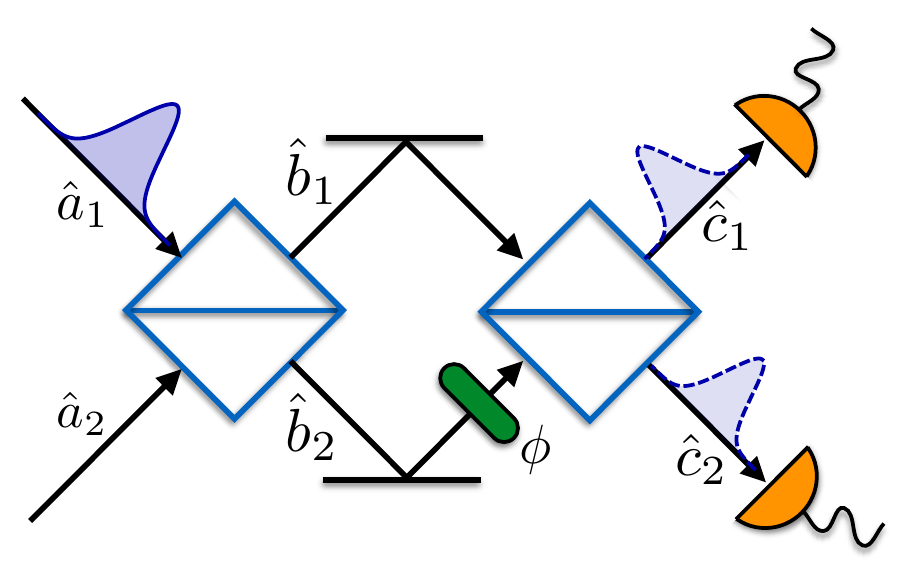
\includegraphics[width=\linewidth]{./gfx/HOM-Phaseshift}
	\begin{minipage}{\linewidth}
		\tiny
		Image Source:\\
		Adam M. Kaufman et al. \enquote{The Hong–Ou–Mandel Effect With Atoms}.
		\emph{Advances In Atomic, Molecular, and Optical Physics (2018)}
	\end{minipage}
\end{columns}
%
\end{frame}

% =========================================================================== %

\begin{frame}[t]{The Hong-Ou-Mandel Effect: Generalization}
%
\begin{columns}
\column{.75\linewidth}
\begin{itemize}
\item Concatenate $\frac{K(K-1)}{2}$ beam splitters with $\frac{K(K-1)}{2}$ phase shifting devices in a pyramidal arrangement
\item Apply same rules to get a $K \times K$ unitary matrix \matU of \emph{single particle transition amplitudes}
	\begin{itemize}
	\item $\ket{j} = \cre_j \vac$
	\item $\ket{k} = \cre[b]_j \vac$
	\item $u_{jk} = \matrixel{j}{\opU}{k}$
	\end{itemize}
\item Particular case: $T = R = \smallfrac{1}{2}$: get DFT matrix
	\begin{align*}
		\matU
	=
		\qty( u_{kl} )_{k, l = 1..K}
	&=
		\frac{1}{\sqrt{K}}
		\qty( \exp(2\pi\iunit \frac{(k-1)(l-1)}{K}) )_{k, l = 1..K}
	\label{eqn:DefDFT}
	\end{align*}
\end{itemize}
%
%
\column{.30\linewidth}
	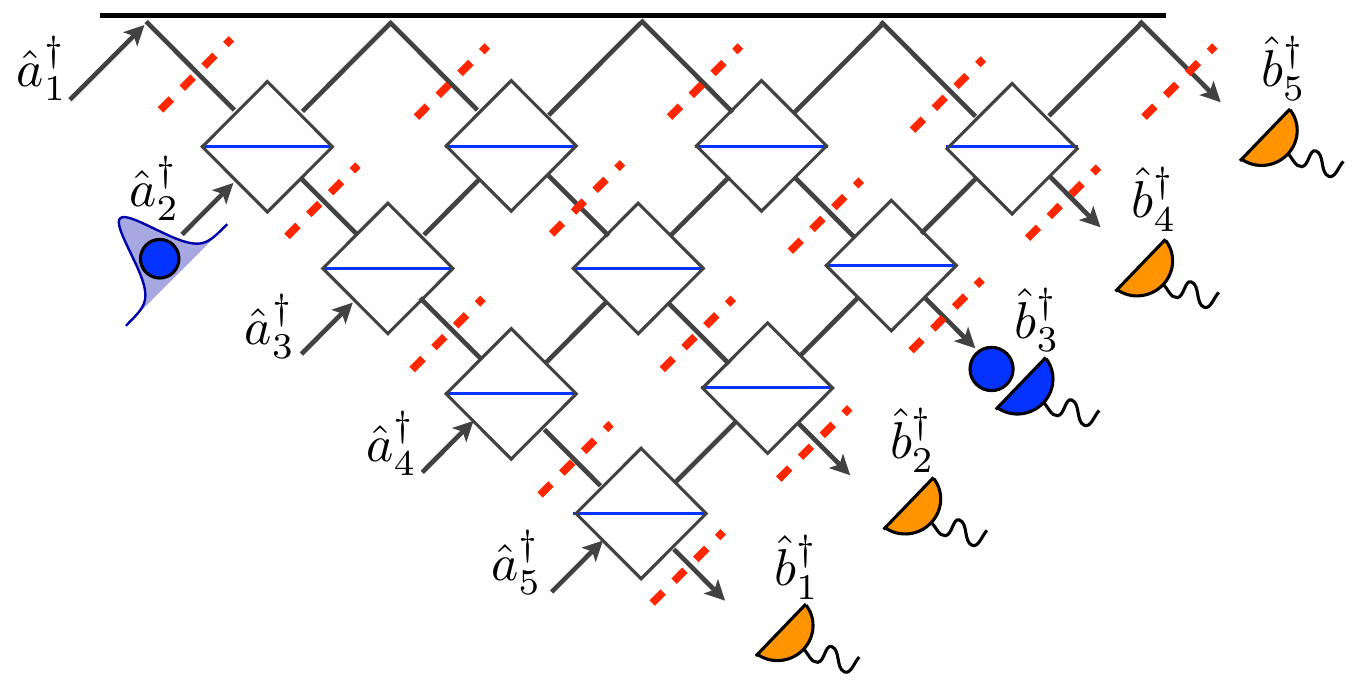
\includegraphics[width=\linewidth]{./gfx/HOM-full}
	\begin{minipage}{\linewidth}
		\tiny
		Image Source:\\
		Malte C. Tichy. \enquote{Interference of Identical Particles from Entanglement to Boson-Sampling}.
		\emph{Journal of Physics B: Atomic, Molecular, and Optical Physics, Volume 47, Issue 10, article id. 103001 (2014)}
	\end{minipage}
\end{columns}
%
\end{frame}

% =========================================================================== %

\begin{frame}{Scattering Amplitudes as Permanents}
%
\begin{itemize}
\item Occupation lists $\vec{m}, \vec{n}$
\item Absorb complexities from equivalent rearrangements into matrix:
	\begin{align*}
			\mathbb{V}
		&\coloneqq
			\qty(v_{ij})_{\substack{
				i=1 \ldots K\\
				j=1 \ldots K
			}}
		&
			v_{ij}
		&\coloneqq
			u_{d_j(\vec{m}), d_k(\vec{n})}
	\end{align*}
\item Retrieve the permanent:
	\begin{equation*}
		P_B(\sysArgs)
	=
		\frac
			{\qty|\perm \mathbb{V}|^2}
			{\prod_{j=1}^K m_j! \; n_j!}
	\end{equation*}
\item For $\vec{m} = \vec{n} = \oplus_{j=1}^K (1)$ and $R = T = \smallfrac{1}{2}$: $\mathbb{V}$ is DFT matrix
\item[\Thus] Know occupation lists $\vec{m}, \vec{n}$, measure probability $P$ to \enquote{compute} the permanent!
\item Difficult to maintain coherence, but in theory possible for arbitrary sizes
\end{itemize}
%
\end{frame}

% =========================================================================== %

\begin{frame}{Scattering Amplitude as Polynomial}
%
\begin{itemize}
\item Scattering Amplitude can be written as
	\begin{align*}
		A(\sysArgs)
	&=
		\eval{\qty(
			\prod_{j=1}^{K}
				\frac
					{1}
					{\sqrt{m_j! \; n_j!}}
				\pdv[m_j]{x_j}
				\pdv[n_j]{y_j}
			) \exp(\vec{x}\transp \, \mathbb{U} \, \vec{y})
		}_{\vec{x} = \vec{y} = \vec{0}}
	\end{align*}
\item Taylor expansion of exponential
\item Evaluate partial derivatives
\item Evaluate $\vec{x} = \vec{y} = \vec{0}$
\item Use $\sum_j m_j = \sum_j n_j = N$
\item Get
	\begin{align*}
		A(\sysArgs)
	&=
		\eval{
			\qty(
				\prod_{j=1}^{K}
					\frac
						{\sqrt{m_j! \; n_j!}}
						{N!}
			)
			\qty( 
				\sum_{r=1}^{K}
				\sum_{c=1}^{L}
					x_r
					y_c
					u_{r,c}
			)^N
		}_{\vec{x} = \vec{y} = \vec{0}}
	\end{align*}
\end{itemize}
%
\begin{minipage}{\linewidth}
\tiny
Source: Thomas Engl, Juan Diego Urbina, and Quirin Hummel, and Klaus Richter.
\enquote{Complex scattering as canonical transformation: A semiclassical approach in Fock space}
\end{minipage}
%
\end{frame}

% =========================================================================== %

\begin{frame}{Scattering Amplitude as Polynomial}
%
\begin{columns}[t]
\column{.5\linewidth}
\vspace{-15pt}
\begin{center}
	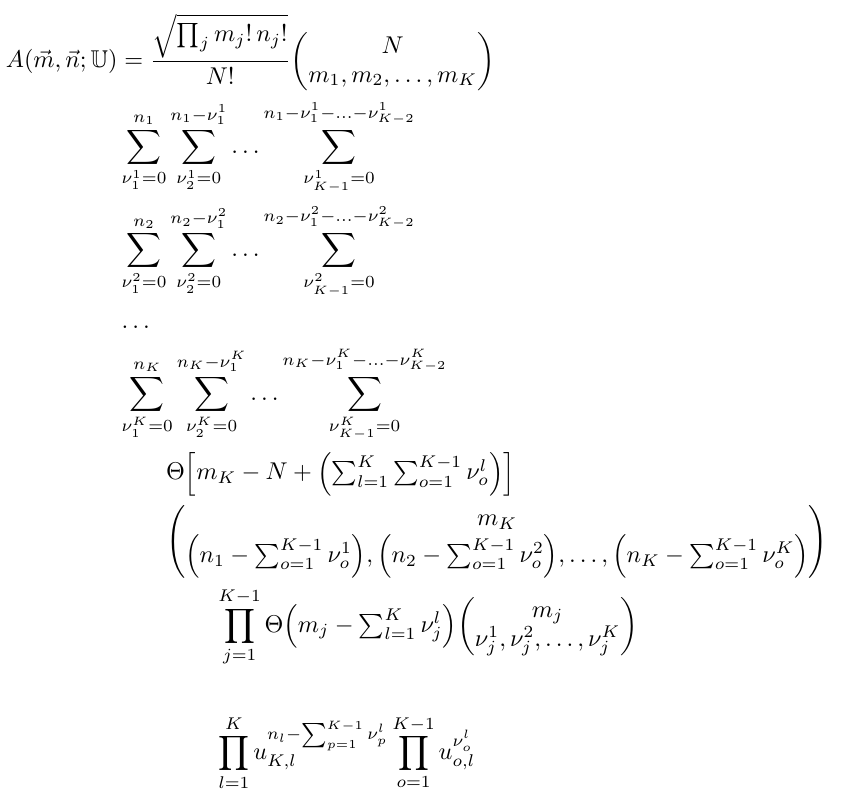
\includegraphics[width=\linewidth]{./gfx/Amplitude-Exact}
\end{center}
%
\column{.5\linewidth}
Recognize Form
\begin{align*}
	A(\sysArgs)
&=
	p(\vec{m}, \vec{n})
	\sum_{\Gamma \in \Xi}
		f(\Gamma, \sysArgs)
\end{align*}
where
\begin{align*}
	p(\vec{m}, \vec{n})
&=
	\frac
		{\sqrt{\prod_j m_j! \, n_j!}}
		{N!}
	\mqty(
		N \\
		m_1, m_2, \ldots, m_K
	)
\end{align*}
and
\begin{gather*}
	\Gamma
=
	\qty( \nu_i^j )
\qquad
	\text{Coefficient matrix}
\\
	\Xi :
	\text{set of all valid coefficient matrices}
\end{gather*}
\end{columns}
%
\end{frame}

% =========================================================================== %

\begin{frame}[fragile]{Runtime Analysis}
%
\begin{columns}[t]
\column{.5\linewidth}
	\begin{itemize}
	\item Coefficient matrix $\Gamma$:
		\begin{itemize}
		\item integer matrices of size $K \times (K - 1)$
		\item matrix elements between $0..N$
		\item[\Thus] $\bigo{N^{K^2}}$ coefficient matrices
		\end{itemize}
	\end{itemize}
%
\column{.5\linewidth}
	\begin{itemize}
	\item Summands $f(\Gamma, \sysArgs)$:
		\begin{itemize}
		\item Triple product symbol
		\item Upper boundary $\leq K$
		\item[\Thus] $\bigo{K^3}$ per summand
		\end{itemize}
	\end{itemize}
\end{columns}
%
\vspace{6pt}
\begin{itemize}
\item[\Thus] $\bigo{K^3 N^{K^2}} = \bigo{N^{3\log_N(K) + K^2}}$ FLOPs
\item Exponential in $K$, polynomial in $N$
\item Note: Ryser Formula for Permanents: $\bigo{2^{n - 1} n^2}$ FLOPs
\end{itemize}
%
\end{frame}

% =========================================================================== %

\begin{frame}{Test of Implementation}
%
\begin{columns}[t]
\column{.7\linewidth}
	\vspace{-20pt}
	\begin{center}
	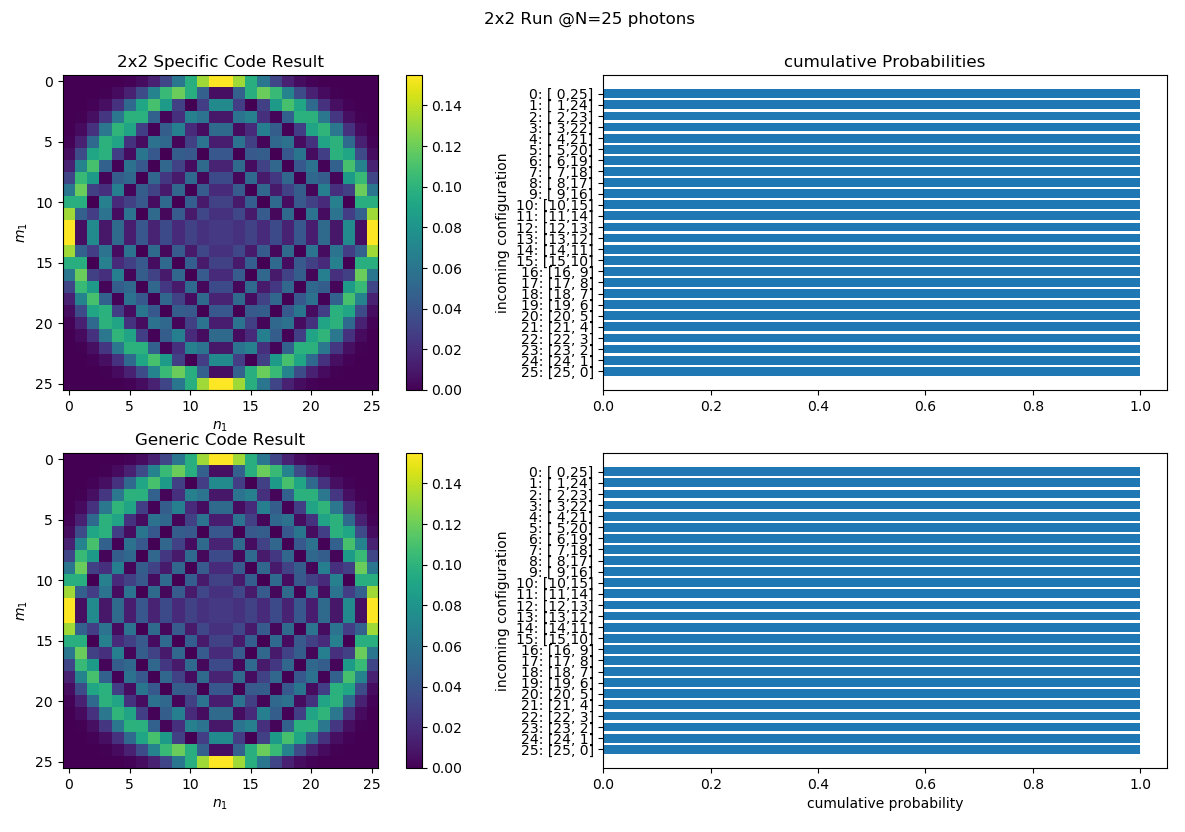
\includegraphics[width=\linewidth]{./gfx/compExact-K2}
	\end{center}

\column{.3\linewidth}
	\begin{itemize}
	\item Check Implementation against specific $2 \times 2$ and $3 \times 3$ code
	\item Use Unitarity: Sum over outcomes must be 1
	\item Symmetry of DFT matrix \Thus Symmetry of Graph
	\item Implementation satisfies tests
	\end{itemize}
\end{columns}
%
\end{frame}

% =========================================================================== %

\begin{frame}{The Scattering Amplitude as Integrals}
%
From previous amplitude formula, with Cauchy's integral formula:
\begin{align*}
	A(\vec{m}, \vec{n})
&=
	(2\pi\iunit)^{-(b_i + b_o)}
	\oint_{\gamma}
		\qty( \prod_{j : m_j \neq 0}
			\frac
				{\sqrt{m_j!} \dd{x_j}}
				{x_j^{m_j+1}}
		)
		\qty( \prod_{k : n_k \neq 0}
			\frac
				{\sqrt{n_k!} \dd{y_k}}
				{ y_k^{n_k+1} }
		)
		\exp( \Big. \vec{x}\transp \, \mathbb{U} \, \vec{y})
\end{align*}

Define curve, interpret as \emph{fixed occupation, all phases}:
\begin{align*}
	\begin{cases}
	x_j &= \sqrt{m_j} \exp( \iunit \theta_j) \\
	y_j &= \sqrt{n_j} \exp(-\iunit \chi  _j)
	\end{cases}
\end{align*}

Where $b_i$: number of incoming occupied modes; $b_o$: number of outgoing occupied modes.
(Zero occupation numbers cancel out; set $\theta_k = 0$ for $m_k = 0$; analogous for $\chi_k, n_k$)
%
\end{frame}

% =========================================================================== %

\begin{frame}{The Scattering Amplitude as Integrals}
%
Select reference mode $j^*$ and integrate out $\theta_{j^*}$. Get:
\begin{align*}
	A(\vec{m}, \vec{n})
=
	2\pi C \,
	\int_{0}^{2\pi}
		\DD{\theta} \DD{\chi}
	&\exp[
		\iunit \qty(
			\vec{n} \cdot \vec{\chi}
			-
			\vec{m} \cdot \vec{\theta}
		)]
\\
	&\exp[
		{\textstyle \sum_{s,t=1}^{K} }
			\sqrt{m_s, n_t} \;
			u_{s,t}
			\exp(\Big. \iunit(\theta_s - \chi_t) )
	]
\end{align*}

Where
\begin{align*}
	C
&\coloneqq
	(-1)^{b_o} \;
	\delta_{M,N} \;
	(2\pi)^{-(b_i + b_o)} \;
	\qty( \prod_{j : m_j \neq 0}
		\sqrt{\frac
			{ m_j! }
			{ m_j^{m_j} }
		}
	)
	\qty( \prod_{k : n_k \neq 0}
		\sqrt{\frac
			{ n_k! }
			{ n_k^{n_k} }
		}
	)
\end{align*}
\begin{align*}
	\DD{\theta}
&\coloneqq
	\prod_{\substack{j : m_j \neq 0 \\ j \neq j^*}}
		\dd{\theta_j}
&
	\DD{\chi}
&\coloneqq
	\prod_{k : n_k \neq 0}
		\dd{\chi  _k}
\end{align*}
%
\end{frame}

% =========================================================================== %

\begin{frame}{Stationary Phase Approximation (SPA)}
%
\begin{align*}
	\oint_{\gamma} \dd[K]{\vec{z}}
		\exp[-\iunit \lambda f(\vec{z})]
&\approx
	\qty( \frac
		{2\pi}
		{\lambda}
	)^{\frac{K}{2}}
	\sum_{r}
		\frac
		{\exp(-\iunit \lambda f(\vec{z}^{(r)}))}
		{\sqrt{\det S^{(r)}}}
\end{align*}

Where
\begin{align*}
	f &: \setComplex^{K} \to \setComplex 													&& \text{arbitrary function} \\
	\lambda & \in \setReals																				&& \text{arbitrary, large} \\
	\vec{z}^{(r)} &: \eval{\grad f}_{\vec{z} = \vec{z}^{(r)}} = 0		&& \text{Saddle Points of } f \\
	S^{(r)} &\coloneqq
		\eval{
		\mqty(
			\pdv{z_i} \pdv{z_j} f
		)_{\substack{
				i=1, \ldots, K\\
				j=1, \ldots, K
			}}
		}_{\vec{z} = \vec{r}^{(r)}}
	&& \text{Hessian matrix of }f
\end{align*}
%
\end{frame}

% =========================================================================== %

\begin{frame}{Applying the SPA}
%
\vspace{-15pt}
\begin{align*}
	A(\vec{m}, \vec{n})
&=
	(-1)^{b_o} \,	
	(2\pi)^{-\frac{(b_i + b_o - 1)}{2}}
	\qty[
		{\Bigg(} \prod_{\substack{j : m_j \neq 0\\j \neq j^*}} m_j {\Bigg)}
		{\Bigg(} \prod_{          k : n_k \neq 0             } n_k {\Bigg)}
	]^{-\smallfrac{1}{2}}
	\exp(N) PT
\end{align*}

where
\begin{align*}
	P
&\coloneqq
	\qty( \prod_{j : m_j \neq 0}
		\sqrt{\frac
			{ m_j! }
			{ m_j^{m_j} }
		}
	)
	\qty( \prod_{k : n_k \neq 0}
		\sqrt{\frac
			{ n_k! }
			{ n_k^{n_k} }
		}
	)
&
	T
&\coloneqq
	\sum_{r}	
		\frac
			{\prod_{k : n_k \neq 0}                  \qty(\nu_k^{(r)})^{n_k}}
			{\prod_{j : m_j \neq 0 \land j \neq j^*} \qty(\mu_j^{(r)})^{m_j}}
		\frac{1}{\sqrt{\Upsilon_r}}
\end{align*}
%
\begin{align*}
	\mu_j
&\coloneqq
	\exp(\iunit \theta_j) \text{ for } m_j \neq 0
&
	\nu_k
&\coloneqq
	\exp(\iunit \chi  _k) \text{ for } n_k \neq 0
\end{align*}
%
\begin{align*}
	\Upsilon(\vec{\mu}, \vec{\nu})
&\coloneqq
	\qty( \prod_{k: n_k \neq 0} \nu_k^{-2} )
		\det\qty[\bigg.
				\diag^2(\vec{\nu})
			-
			\tilde{\mathbb{U}}\transp
			\diag^2(\vec{\mu})
			\tilde{\mathbb{U}}
		]
\end{align*}
%
\end{frame}

% =========================================================================== %

\begin{frame}{Stirling Approximation}
%
\begin{itemize}
\item Factor $P$ comprises of terms of form $\sqrt{\smallfrac{k!}{k^k}}$ with $k \in \setNaturals$
%\item Big numbers out of int-range for processors, need to be treated as floating point numbers early on (or use big integer libraries)
%\item Acquire big numerical errors
\item Stirling's approximation:
	\begin{equation*}
		k! \approx \sqrt{2\pi k} \exp(-k) k^k
	\end{equation*}
\item Get rid of $\frac{k^k}{k^k}$ in $P$, get expression for scattering amplitude:
	\begin{align*}
		A(\vec{m}, \vec{n})
	&=
		(-1)^{b_o} \,	
		(2\pi)^{-\frac{b_i + b_o - 2}{4}}
		\sqrt{m_{j^*}}
		\lambda^{-\smallfrac{1}{4}}
		\sum_{r}	
			\frac
				{\prod_{k : n_k \neq 0}                  \qty(\nu_k^{(r)})^{n_k}}
				{\prod_{j : m_j \neq 0 \land j \neq j^*} \qty(\mu_j^{(r)})^{m_j}}
			\frac{1}{\sqrt{\Upsilon_r}}
		\\
			\lambda
		&\coloneqq
			\qty( \prod_{j : m_j \neq 0} m_j )
			\qty( \prod_{k : n_k \neq 0} n_k )
	\end{align*}
\end{itemize}
%
\end{frame}

% =========================================================================== %

\begin{frame}{Saddle Point Condition}
%
\begin{gather*}
	\pdv{f}{\theta_p}
=
	\iunit \lambda^{-1}
	\qty[
		m_p
		-
		\sum_{l=1}^{K}
			\sqrt{m_p n_l} \; u_{p,l} \; \exp[ \Big. \iunit(\theta_p - \chi_l)]
	]
=
	0 \\
\Thus
	\sqrt{m_p} \exp(-\iunit \theta_p)
=
	\sum_{l=1}^{K} \sqrt{n_l} \; u_{p,l} \; \exp(-\iunit\chi_l)
\end{gather*}
%
\vspace{6pt}
\begin{center}
	or, briefly:
\end{center}
\vspace{6pt}
%
\begin{equation*}
	\vec{x}^{*} = \mathbb{U} \vec{y}
\end{equation*}
%
\end{frame}

% =========================================================================== %

\begin{frame}{Finding The Saddle Points: Phase Retrieval}
%
\begin{itemize}
\item Problem Statement: Phase Retrieval Problem
	\vspace{-10pt}
	\begin{columns}[t]
	\column{.4\linewidth}
	\begin{itemize}
	\item Let there be functions $f(x), \hat{f}(\omega)$
	\item $\hat{f}(\omega) = \mathcal{F}_x[f]$ : Fourier pair
	\end{itemize}
	%
	\column{.5\linewidth}
	\begin{itemize}
	\item Known are only modulus data $F, \hat{F}$
	\item $F(x) = \abs{f(x)}$ and $\hat{F}(\omega) = \abs{\hat{f}(x)}$
	\end{itemize}
	\end{columns}
	
\item[\Thus] Find a function $\theta: \setReals \to \setReals$ such that $f(x) = \exp(\Big. \iunit \theta(x)) F(x)$
\item Discretized version
	\begin{itemize}
	\item $f(x) \to \vec{f}$ where $f_k = f(x_k)$ and $x_k = j \Delta x$
	\item $\mathcal{F}_x : \hat{\vec{f}} = \mathbb{W} \vec{f}$
	\item $\mathbb{W}$: DFT matrix (\ie \matU)
	\item $F_j, \hat{F}_j$: square roots of occupation lists ($x_j = \sqrt{m_j}, y_j = \sqrt{n_j}$)
	\end{itemize}
\end{itemize}
%
\end{frame}

% =========================================================================== %

\begin{frame}{Finding The Saddle Points: Phase Retrieval}
%
\begin{itemize}
\item Start with an initial guess $\theta^{(0)}(x)$ and define $f^{(0)}(x) = F(x) \exp(\Big.\iunit \theta^{(0)}(x))$
\item Iteratively compute
	\begin{align*}
		\hat{f}^{(k)}(\omega) &= \mathcal{F}_x f^{(k)}(x)
	&
		\hat{\vec{f}}^{(k)} &= \mathbb{W} \vec{f}^{(k)}
\\
		\hat{f}^{(k + 1)}(\omega)
	&=
		\hat{F}(\omega)
		\frac
			{ \hat{f}^{(k)}(\omega) }
			{|\hat{f}^{(k)}(\omega)|}
	&
		\hat{f}^{(k + 1)}_j
	&=
		\hat{F}_j
		\frac
			{ \hat{f}^{(k + 1)}_j }
			{|\hat{f}^{(k + 1)}_j|}
\\
		\tilde{f}^{(k + 1)}(x) &= \mathcal{F}^{-1}_x  f^{(k)}(x)
	&
		\tilde{\vec{f}}^{(k + 1)} &= \mathbb{W}^{-1} \vec{f}^{(k + 1)}
\\
		f^{(k + 1)}(x)
	&=
		F(x)
		\frac
			{ \tilde{f}^{(k + 1)}(x) }
			{|\tilde{f}^{(k + 1)}(x)|}
	&
		f^{(k + 1)}_j
	&=
		F_j
		\frac
			{ \tilde{f}^{(k + 1)}_j }
			{|\tilde{f}^{(k + 1)}_j|}
	\end{align*}
\item When converged, extract phase
	\begin{align*}
		\theta^{(k + 1)}(x) &= \arg\qty(f^{(k + 1)})(x)
	&
		\theta^{(k + 1)}_j &= \arg\qty(f^{(k + 1)})_j
	\end{align*}
\end{itemize}
%
\end{frame}

% =========================================================================== %

\begin{frame}{Finding All Solutions}
%
\begin{itemize}
\item Different $\vec{\theta}^{(0)}$ gives different solution
\item Brute Force exploration of $K$-dimensional space of initial guesses
\end{itemize}
%
\begin{minipage}{\linewidth}
	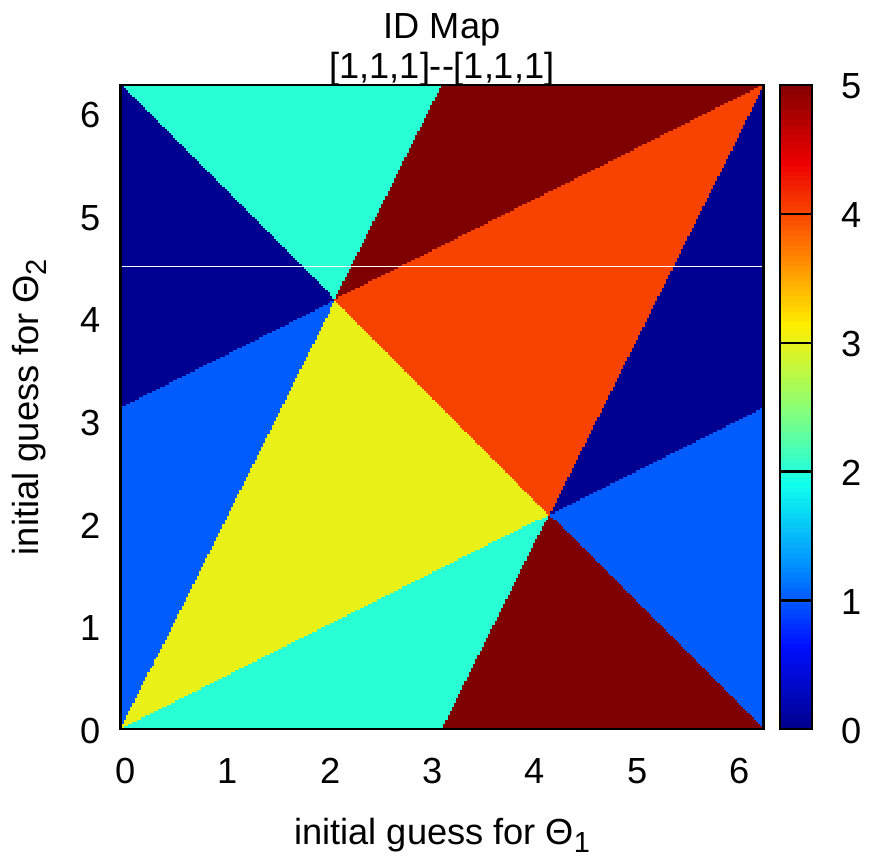
\includegraphics[width=.32\linewidth]{./gfx/IDmap-K3}
	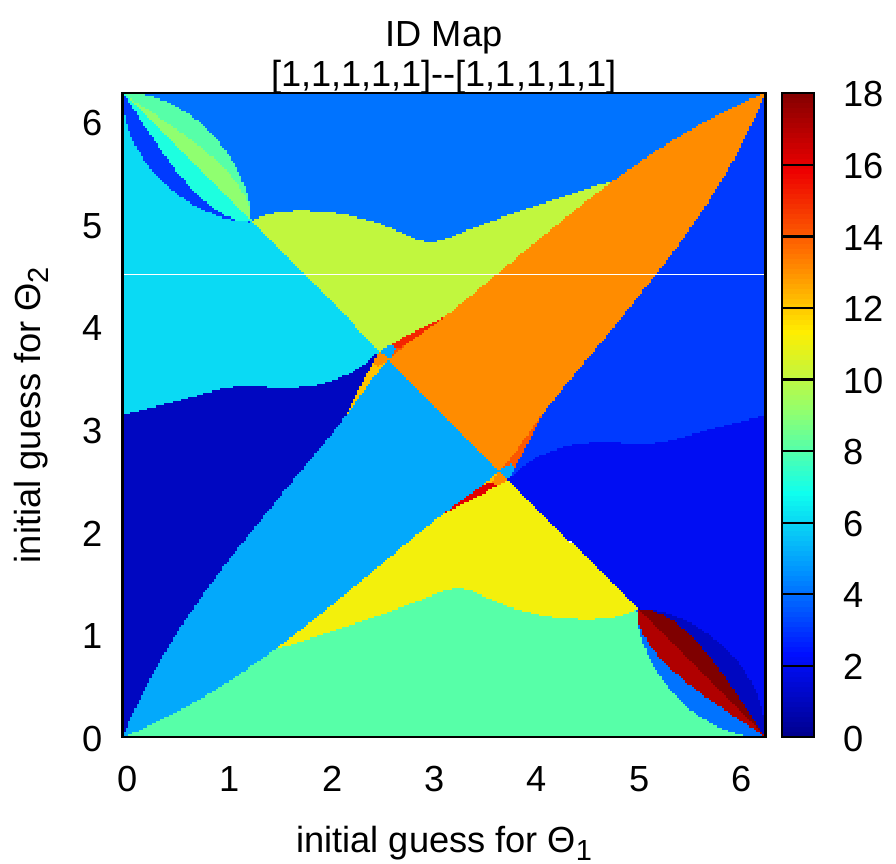
\includegraphics[width=.32\linewidth]{./gfx/IDmap-K5}
	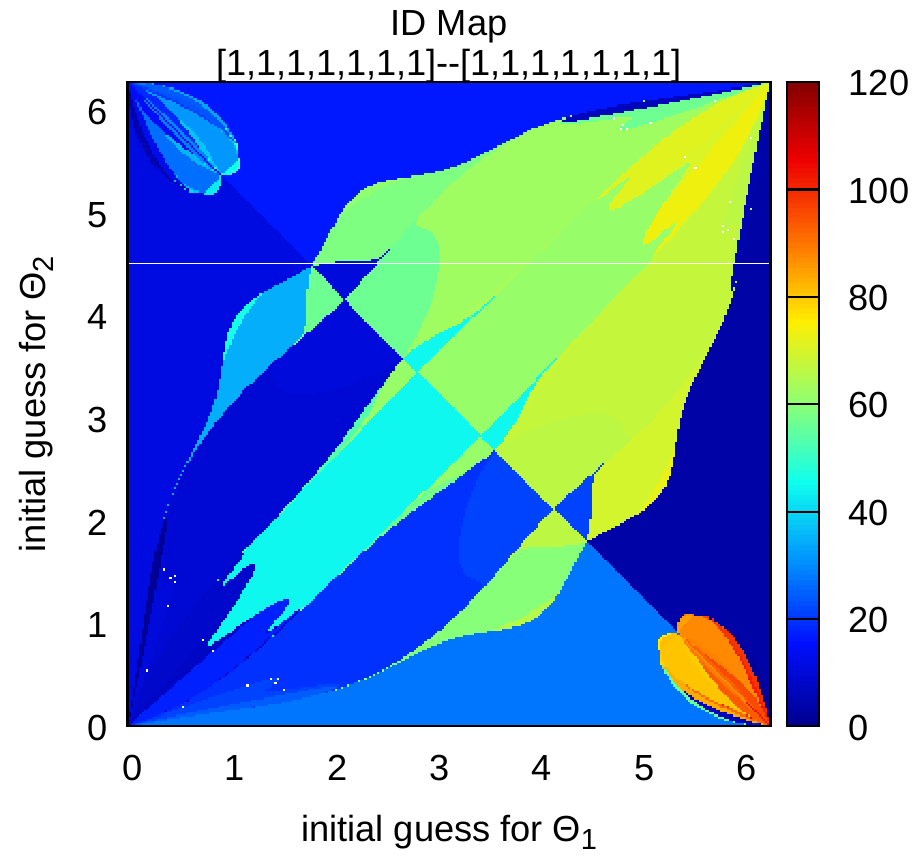
\includegraphics[width=.32\linewidth]{./gfx/IDmap-K7}
\end{minipage}
%
\end{frame}

% =========================================================================== %

\begin{frame}{Implementation: Structure of PRA}
%
\begin{columns}[t]
\column{.65\linewidth}
\vspace{-20pt}
\begin{center}
	\includegraphics[width=\linewidth]{./gfx/Scheme-PRA}
\end{center}
%
\column{.4\linewidth}
\begin{itemize}
\item Input: \texttt{.ini} file (pairs in form \texttt{key = value})
%	\begin{itemize}
%	\item Number of photons and modes
%	\item List of occupation lists
%	\item Sweep description
%	\item Filter parameters
%	\item Output file specifications
%	\end{itemize}
\item Parallelized Processing, variable number of threads
\item Output:
	\begin{itemize}
	\item Phaselists
	\item ID- and Iteration-maps
	\end{itemize}
\end{itemize}
\end{columns}
%
\end{frame}

% =========================================================================== %

\begin{frame}[fragile]
%
\begin{columns}[t]
\column{.35\linewidth}
\phantom{x}

\vspace{6pt}
\begin{Large}
	Settings Files
\end{Large}
\vspace{12pt}
%
\begin{itemize}
\item Definition of multiple occupations
\item Definition of initial guesses
\item Different kinds of maps and lists
\item Plotting Parameters
\item Filter Parameters
\end{itemize}
%
\column{.65\linewidth}
\begin{minted}[fontsize=\tiny]{ini}
N_modes   = 3
N_photons = 4
threads   = 4

# possible values for keyword_occupation: NONZERO, EQUAL, ALL
keyword_occupation      = NONZERO

# possible values for keyword keyword_initial_guess: SWEEP, SINGLE
keyword_initial_guess   = SWEEP
parameter_initial_guess = 0:2PI

# possible values for mission:
#   FINDUNIQUE,
#   MAKEPHASELIST, MAKEVECTORLIST,
#   MAKEIDMAP, MAKEITERMAP, MAKECONVERGENCEMAP, MAKESUCCESSMAP,
#   MAKEEFFORTMAP, MAKEERRORCOUNTMAP, MAKESOLUTIONCOUNTMAP
mission         = FINDUNIQUE, MAKEVECTORLIST, MAKEERRORCOUNTMAP, MAKEIDMAP
outputformat    = TXT, GNUPLOT, PDF
plotdimensions  = AUTO
plotslice       = AUTO

filename_directory = ./output/
filename_prefix = sweep2D_K=3_N=4
filename_midfix = EXPLICIT
filename_suffix = :201; 0:2PI:201; 3.1415

epsilon_convergence = 1E-6
epsilon_backtest    = 1E+1
epsilon_unique      = 1E-3
max_iterations      = 1500
\end{minted}
\end{columns}
%
\end{frame}

% =========================================================================== %

\begin{frame}{Implementation: Structure of SPA}
%
\vspace{-15pt}
\begin{columns}[t]
\column{.7\linewidth}
\begin{center}
	\includegraphics[width=\linewidth]{./gfx/Scheme-SPA}
\end{center}
%
\column{.3\linewidth}
\begin{itemize}
\item Input: Settings file, plus phaselist CSV(s)
\item Computation of scattering amplitudes for a number of scattering problems $\vec{m}^{(l)} \to \vec{n}^{(l)}$ in a single run
\item Output: Again: CSVs, PDFs
\item Several Reports: SPA result, exact amplitude (polynomial formula), difference, map of error codes
\end{itemize}
\end{columns}
%
\end{frame}

% =========================================================================== %

\begin{frame}{Results}
%
\begin{minipage}{.49\linewidth}
	\includegraphics[width=\linewidth]{./gfx/Probabilty-K2-Exact}
\end{minipage}
%
\begin{minipage}{.49\linewidth}
	\includegraphics[width=\linewidth]{./gfx/Probabilty-K2-SPA}
\end{minipage}
%
\begin{columns}[t]
\column{.5\linewidth}
\begin{itemize}
\item Number of modes $K = 2$
\item Number of photons $N = 25$
\item No zero occupancies
\end{itemize}
%
\column{.5\linewidth}
\begin{itemize}
\item Very good results \enquote{in the center}\\
	(where $m_j, n_j$ are big)
\item Finds all zeros
\end{itemize}
\end{columns}
%
\end{frame}

% =========================================================================== %

\begin{frame}{Difference: SPA vs. Exact}
%
\begin{columns}
\column{.6\linewidth}
	\includegraphics[width=\linewidth]{./gfx/Probabilty-K2-DeltaRelative}
%
\column{.4\linewidth}
	\begin{itemize}
	\item Axes: Configuration
		\begin{itemize}
		\item $x$: Outgoing
		\item $y$: Incoming
		\end{itemize}
	\item Relative Difference of Transition Probabilities
		$
			\frac
				{\left| \big. [\text{Probability SPA}] - [\text{Probability Exact}] \right|}
				{[\text{Probability Exact}]}
		$
	\item Zeros predicted correctly
		\begin{itemize}
		\item[\Thus] Interference modelled correctly!
		\end{itemize}
	\item Bad results on the boundaries
		\begin{itemize}
		\item Expected -- $\lambda$ parameter small
		\end{itemize}
	\end{itemize}
\end{columns}
%
\end{frame}

% =========================================================================== %

\begin{frame}{Results}
%
\begin{minipage}{.49\linewidth}
	\includegraphics[width=\linewidth, page=1]{./gfx/Probabilty-K3-Exact}
\end{minipage}
%
\begin{minipage}{.49\linewidth}
	\includegraphics[width=\linewidth, page=2]{./gfx/Probabilty-K3-Exact}
\end{minipage}
%
\begin{columns}[t]
\column{.5\linewidth}
\begin{itemize}
\item Number of modes $K = 3$
\item Number of photons $N = 12$
\item Includes zero occupancies
\end{itemize}
%
\column{.5\linewidth}
\begin{itemize}
\item Runs with different filter settings
\item About 20 min computation time per run
\item (4 threads, CIP pool computers via SSH)
\end{itemize}
\end{columns}
%
\end{frame}

% =========================================================================== %

\begin{frame}
%
\begin{columns}[b]
\column{.7\linewidth}
	\includegraphics[width=\linewidth, page=1]{./gfx/Probabilty-K3-1-SPA}
%
\column{.3\linewidth}
	\includegraphics[width=\linewidth, page=1]{./gfx/Probabilty-K3-1-Rel}
	
	\begin{itemize}
	\item Some characteristic patterns reproduced
	\item Many bad data points
	\item Accumulated probabilites \emph{in a reasonable range}
	\end{itemize}
\end{columns}
\begin{itemize}
\item[\Thus] Actually best of several filter settings
\end{itemize}
%
%
% used: K3-1: "run 03" in pull directory
% epsilon_convergence = 1E-2
% epsilon_backtest    = 5E-2
% epsilon_unique      = 1E+1
% max_iterations      = 300
%
% used: K3-2: "run 10" in pull directory
% epsilon_convergence = 1E-3
% epsilon_backtest    = 1E+1
% epsilon_unique      = 1E-3
% max_iterations      = 300
%
\end{frame}

% =========================================================================== %

\begin{frame}
%
\begin{minipage}{.49\linewidth}
	\includegraphics[width=\linewidth, page=1]{./gfx/Probabilty-K3-1-SPA}
\end{minipage}
%
\begin{minipage}{.49\linewidth}
	\includegraphics[width=\linewidth, page=1]{./gfx/Probabilty-K3-1-Rel}
\end{minipage}
%
\begin{minipage}{.49\linewidth}
	\includegraphics[width=\linewidth, page=1]{./gfx/Probabilty-K3-2-SPA}
\end{minipage}
%
\begin{minipage}{.49\linewidth}
	\includegraphics[width=\linewidth, page=1]{./gfx/Probabilty-K3-2-Rel}
\end{minipage}
%
% used: K3-1: "run 03" in pull directory
% epsilon_convergence = 1E-2
% epsilon_backtest    = 5E-2
% epsilon_unique      = 1E+1
% max_iterations      = 300
%
% used: K3-2: "run 10" in pull directory
% epsilon_convergence = 1E-3
% epsilon_backtest    = 1E+1
% epsilon_unique      = 1E-3
% max_iterations      = 300
%
\end{frame}

% =========================================================================== %

\begin{frame}{Parameters}
%
\begin{itemize}
\item \texttt{max\_iterations} -- how many iterations to compute at most
\item \texttt{epsilon\_convergence} -- demand $\norm{\vec{x} - \text{PRA}(\vec{x})} < \varepsilon_{\text{conv}}$ to even consider a state as a solution
	\begin{itemize}
	\item Too big -- will find wrong solutions
	\item Too small -- increases computation time, might not converge at all
	\end{itemize}
\item \texttt{epsilon\_backtest} -- demand $\norm{\vec{x}^* - \matU \vec{y}} < \varepsilon_{\text{back}}$
	\begin{itemize}
	\item Loops are possible
	\item Pathologic cases involving zero occupancies
	\end{itemize}
\item \texttt{epsilon\_unique} -- demand $\norm{\vec{\theta}^{(r)} - \vec{\theta}^{\text{new}}} > \varepsilon_{\text{unique}}$
\end{itemize}
%
\end{frame}

% =========================================================================== %

\begin{frame}{Conclusion}
%
Proof of concept
	\begin{itemize}
	\item Mapped a QM interference problem onto the (classical) phase retrieval problem
	\item Problem of multiplicity of solutions is actually part of the solution!
	\item Interference of photons dictates the probability
	\item \emph{All paths taken}
	\end{itemize}

\vspace{6pt}
Further work needed
	\begin{itemize}
	\item Best fit parameters for each scenario
	\item Better ways of detecting correct and unique solutions
	\item Intelligent choice of reference mode
	\end{itemize}
%
\end{frame}

% =========================================================================== %

\begin{frame}{Thank you very much for your attention!}
%
\begin{center}
	%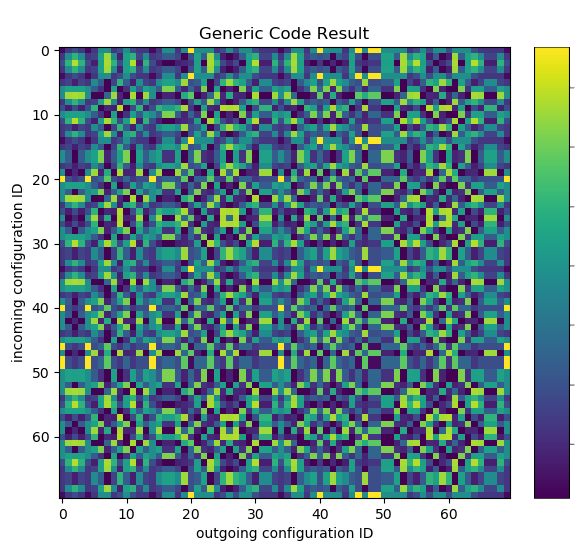
\includegraphics[width=.4\linewidth]{./gfx/Amp-K5-N4}
	% trim=left bottom right top
	\includegraphics[width=.8\linewidth, page=1, trim=0 0 0 10, clip]{./gfx/Probabilty-K3-Exact}
\end{center}
%
\end{frame}

% =========================================================================== %
% APPENDIX
% =========================================================================== %

\setcounter{framenumber}{0}
\begin{frame}{Scattering Amplitudes as Permanents}
%
\begin{itemize}
\item Transition Probability (acessible experimentally):
	$P(\sysArgs) = |A(\sysArgs)|^2$
\item Introduce \emph{Mode Assignment List} $\vec{d}$
	\begin{itemize}
	\item \enquote{Where to find the $d_i^{\text{th}}$ photon}
	\item 
		$\vec{d}(\vec{q}) = \oplus_{j=1}^{K} \oplus_{k=1}^{q_j}(j)
		= (
			\underbrace{1, \ldots, 1}_{q_1\;\text{times}},
			\underbrace{2, \ldots, 2}_{q_2\;\text{times}}, 
			\ldots, 
			\underbrace{K, \ldots, K}_{q_K\;\text{times}}
		  )$
	\end{itemize}
\item Distinguishable particles in order:
	\tabto{1.6cm}
	$P_{\text{ord, dist}}(\sysArgs)
=
	\qty|
		\prod_{j=1}^N
			u_{d_j(\vec{m}), d_j(\vec{n})}
	|^2$
\item Sum over equivalent outcomes:
	\tabto{1.6cm}
	$P_{\text{acc, dist}}(\sysArgs)
= 
	\sum_{\sigma \in S_{\vec{d}(\vec{n})}}
	\qty|
		\prod_{j=1}^N
			u_{d_j(\vec{m}), \sigma(j)}
	|^2$
\item Indistinguishable bosons:
	\tabto{1.6cm}
	$P_B(\sysArgs)
=
	\frac
		{\prod_{j=1}^K n_j!}
		{\prod_{j=1}^K m_j!}
	\qty|
		\sum_{\sigma \in S_{\vec{d}(\vec{n})}}
		\prod_{j=1}^N
			u_{d_j(\vec{m}), \sigma(j)}
	|^2$
\end{itemize}
%
\end{frame}

% =========================================================================== %

\begin{frame}{Scattering Amplitude as Polynomial}
%
\begin{itemize}
\item Use Multinomial Theorem:
	\begin{align*}
		\qty(
			\sum_{l=1}^{m} x_l
		)^{n}
	&=
		\sum_{\substack{\sum_{l=1}^m k_l = n \\ k_l \geq 0}}
		\begin{pmatrix}
			n \\ k_1, k_2, \ldots, k_m
		\end{pmatrix}
		\prod_{t=1}^{m}
			x_t^{k_t}
	&
	\text{where}
	&&
		\begin{pmatrix}
			n \\ k_1, k_2, \ldots, k_m
		\end{pmatrix}
	&=
		\frac{n!}
		{\prod_{l=1}^m k_l !}
	\end{align*}
\item Get closed form expression for exact scattering amplitude
\end{itemize}
%
\end{frame}

% =========================================================================== %

\begin{frame}{Implementation: Structure of File Output Package}
%
\begin{columns}[t]
\column{.7\linewidth}
\begin{center}
	\includegraphics[width=\linewidth]{./gfx/Scheme-FO}
\end{center}
%
\column{.3\linewidth}
\begin{itemize}
\item Input: \texttt{std::span<T>} (non-owning view of contiguous memory, compatible with \texttt{std::vector<T>}
\item Output: CSV-like \texttt{.txt} files, gnuplot scripts, \texttt{.pdf} plots
\end{itemize}
\end{columns}
%
\end{frame}
\setcounter{framenumber}{31}

\end{document}